%
%RESULTS Rev1: Notebook Rev1_13 - A Median & Average Runtime
%median/mean
%LdF_N1_64_W100_Def     19.949113	64.842078
%LdF_N3_64_W100_Def     58.365978 	122.960265
%LdF_N1_64_W1000_Def    300.0		219.935204
%LdF_N3_64_W1000_Def    300.0		216.525390
%
%RESULTS Rev1: Notebook Rev1_13 - B Errors & Timeout percentage
%Fus_N1_64_W100_Def:	Success: 65.0	Error: 0.0	Timeout: 34.9
%Flu_N3_64_W100_Def:	Success: 0.0	Error: 0.0	Timeout: 0.0
%LdF_N1_64_W100_Def:	Success: 89.0	Error: 0.0	Timeout: 10.9
%LdF_N3_64_W100_Def:	Success: 75.2	Error: 0.0	Timeout: 24.7
%
%Fus_N1_64_W1000_Def:	Success: 0.0	Error: 0.0	Timeout: 0.0
%Flu_N1_64_W1000_Def:	Success: 95.0	Error: 0.0	Timeout: 5.0
%Flu_N3_64_W1000_Def:	Success: 0.0	Error: 0.0	Timeout: 0.0
%LdF_N1_64_W1000_Def:	Success: 28.8	Error: 0.0	Timeout: 71.1
%LdF_N3_64_W1000_Def:	Success: 29.3	Error: 0.0	Timeout: 70.6
%

\begin{figure}[htbp!]
\centering
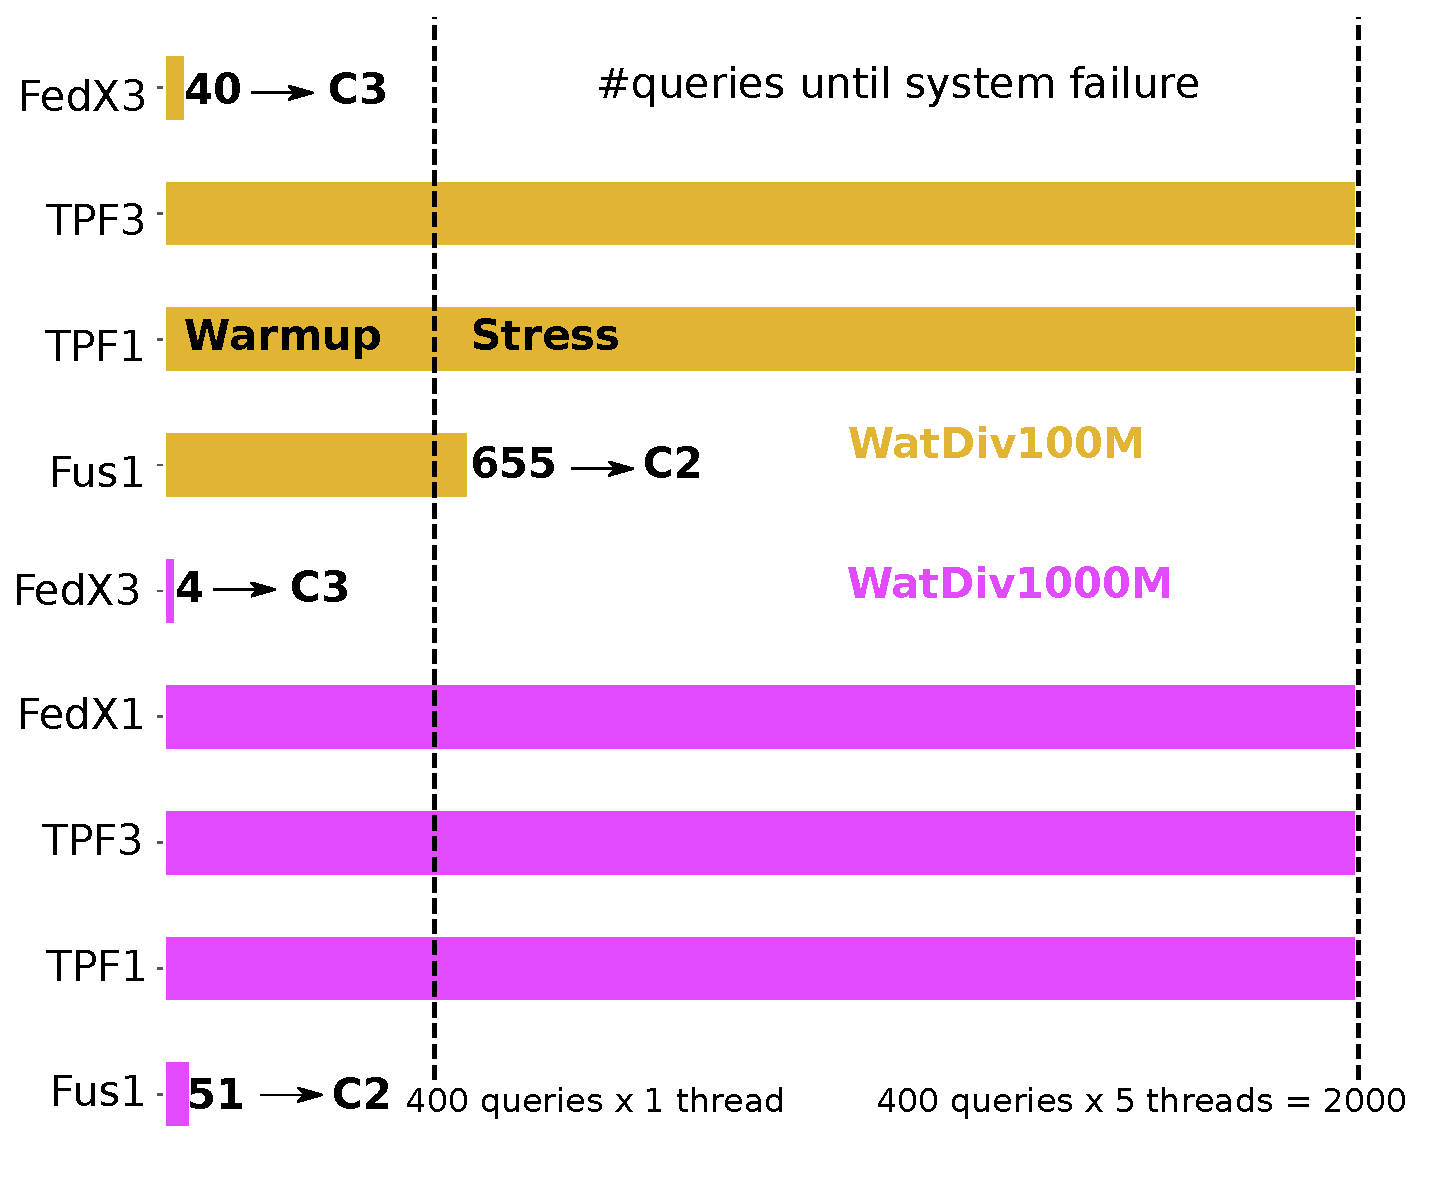
\includegraphics[width=0.99\linewidth]{imgs/Fig03_BenchmarkSurvival_Other_Watdiv_Default}
\caption{Benchmark survival interval for 3 \emph{SemWeb} solutions. For early crashes the amount of queries until system failure is reported, as well as the query template causing the failure. \textbf{Flu3\_64} crashes upon the first occurrence of a \textbf{C3} query. \textbf{Fus1\_64} survives the warm-up run for WatDiv100M but crashes upon the first occurrence of a \textbf{C2} query in the stress test, for WatDiv1000M again the first \textbf{C2} query in the warm-up run causes the crash.}
\label{fig:Fig03_BenchmarkSurvival_Other_Watdiv_Default}
\end{figure}

As the initial goal of the research collaboration with Ontoforce was to find a solution to work with federated querying on top of live data sources on the Semantic Web, we discuss the results of \textbf{Fus1\_64}, \textbf{Flu3\_64}, \textbf{TPF1\_64} and \textbf{TPF3\_64}. 
Figure~\ref{fig:Fig03_BenchmarkSurvival_Other_Watdiv_Default} deliberately has no relation with query runtimes. For these 3 systems engine failure and query errors are very common with only the \textbf{TPF*\_64} systems surviving the entire benchmark. 
\begin{itemize}
	\item \textbf{Flu1\_64:} The federation system with 1 source node is added to verify that FedX in fact manages to parse the queries.
	\item \textbf{Specific Templates cause crashes:} Where \\ \textbf{TPF*\_64} systems more gracefully timeout on the \textbf{C} templates, \textbf{C2} causes a crash in \textbf{Fus1\_64} and \textbf{C3} in \textbf{Flu3\_64}, upon their first occurrence in warm-up or stress run. \textbf{C3} is a query with very low triple pattern selectivity leading to large in-memory joins.
	\item \textbf{Crash investigation:} For \textbf{Flu3\_64} the benchmark was terminated after running into constant timeouts for 8 hours. Upon inspection of the slave nodes (VOS), these turned out to be idle, while the federator node had its entire memory pool saturated, with the CPU load close to zero. A possible explanation might therefore point in the direction of issues with garbage collection.
	For \textbf{Fus1\_64} after a number of queries a continuous timeout sequence sets in. Peculiar was that the specific HDT implementation for Fuseki seemed to ignore the timeout parameter which might explain why the server overloaded and became unresponsive.
	\item \textbf{Staying alive:} \textbf{TPF*\_64} survive both WatDiv benchmarks, nonetheless up to 71\% of the queries timeout for WatDiv1000M. For WatDiv100M the timeout ratio drops to 25\% for \textbf{TPF3\_64} and to 11\% for \textbf{TPF1\_64}.
%Fus_N1_64_W100_Def:	Success: 65.0	Error: 0.0	Timeout: 34.9
%Flu_N3_64_W100_Def:	Success: 0.0	Error: 0.0	Timeout: 0.0
%LdF_N1_64_W100_Def:	Success: 89.0	Error: 0.0	Timeout: 10.9
%LdF_N3_64_W100_Def:	Success: 75.2	Error: 0.0	Timeout: 24.7
%
%Fus_N1_64_W1000_Def:	Success: 0.0	Error: 0.0	Timeout: 0.0
%Flu_N1_64_W1000_Def:	Success: 95.0	Error: 0.0	Timeout: 5.0
%Flu_N3_64_W1000_Def:	Success: 0.0	Error: 0.0	Timeout: 0.0
%LdF_N1_64_W1000_Def:	Success: 28.8	Error: 0.0	Timeout: 71.1
%LdF_N3_64_W1000_Def:	Success: 29.3	Error: 0.0	Timeout: 70.6
	\item \textbf{Runtime Comparison: } Only for WatDiv100M comparing the runtimes of \textbf{TPF*\_64} to the \emph{Vendor} systems is meaningful due to the higher query success rates. Compared to \textbf{ES1\_32}, the \textbf{TPF1\_64} is 2.4 times faster in terms of median runtime and 12\% in terms of batch time. For \textbf{TPF3\_64} the results are worse than \textbf{ES1\_32}: 25\% slower in median runtime, 40\% slower for batch.
\end{itemize}
%Bla_N1_32_W100_Def   0.191359		0.461707
%Gra_N1_32_W100_Def   0.047812		0.417214
%Es_N1_32_W100_Def    48.305706		72.994550
%Vir_N1_32_W100_Def   0.046707		0.301350
%LdF_N1_64_W100_Def     19.949113	64.842078
%LdF_N3_64_W100_Def     58.365978 	122.960265









